\subsection{O que é aprendizagem de máquina?}

Aprendizagem de máquina é a área da ciência da computação que tem como objetivo geral o desenvolvimento de programas
de computador capazes de aprender a realizar uma tarefa sem serem explicitamente programados \cite{Bi2019, Theobald2021}.
Neste contexto, aprendizagem refere-se a aplicação de procedimentos estatísticos e computacionais sobre um conjunto
de informações empíricas, buscando alcançar melhorias de desempenho em uma determinada tarefa \cite{Theobald2021}.

Aprender trata-se, portanto, de ajustar os parâmetros de um modelo estatístico e computacional aos dados observados
de modo a maximizar o desempenho na tarefa em questão. Esse processo de aprendizagem é comumente chamado de treinamento
do modelo \cite{Bi2019}. Programas de computador baseados em aprendizagem de máquina são capazes de identificar padrões
de interação complexos entre variáveis em conjuntos de dados com alta dimensionalidade para realizar tarefas de classificação,
regressão, agrupamento e outras \cite{Theobald2021}.

Considere, por exemplo, um estudo observacional hipotético que investiga a relação entre características de personalidade
e o nível de satisfação profissional entre psicólogos. O estudo baseia-se no modelo dos cinco grandes fatores da personalidade
\cite{Hutz2018} e usa o instrumento da Bateria Fatorial da Personalidade para coleta de dados, registrando as pontuações obtidas
nas escalas de neuroticismo, extroversão, socialização, realização e abertura \cite{Sancineto2015}. Além disso, os participantes
do estudo reportam o próprio nível de satisfação profissional em uma escala que contém os seguintes valores: baixo, médio e alto.

É possível utilizar esse conjunto de dados para construir um modelo de apredizagem de máquina preditivo. Um algoritmo processa o conjunto de dados,
identificando os padrões de interação existentes entre as variáveis preditoras (características de personalidade) e o desfecho de interesse (nível
de satisfação profissional). O conhecimento adquirido durante o processamento dos dados é codificado nos parâmetros de um modelo de aprendizagem de
máquina. O modelo pode então ser utilizado para fazer predições sobre o nível de satisfação profissional de um indivíduo qualquer a partir de suas
características de personalidade.

\subsection{Os tipos de aprendizagem de máquina}
As técnicas de aprendizagem de máquina podem ser organizadas de diferentes maneiras, incluindo classificação pela estratégia adotada durante o processo
de aprendizagem e pelo objetivo geral de aprendizagem \cite{Theobald2021, Ng2001}.

\subsubsection{Aprendizagem supervisionada, não supervisionada e por reforço}
As categegorias mais comumente usadas na descrição de modelos de aprendizagem de máquina dizem respeito à estratégia de aprendizagem adotada. O
modelo pode ser construído segundo uma abordagem de aprendizagem supervisionada, aprendizagem não supervisionada ou aprendizagem por reforço
\cite{Theobald2021, Bi2019}.

A aprendizagem supervisionada assemelha-se ao processo de aprendizagem adotado por seres humanos, onde o aprendiz identifica padrões a partir de
um conjunto de exemplos preparado por um tutor. Durante a fase de aprendizagem, o modelo é exposto a um conjunto de dados que contém informações
sobre o desfecho de interesse para cada uma das observações. O acesso às informações de desfecho providas por um agente externo confere o caráter
de supervisão a este processo. Técnicas de aprendizagem de máquina para regressão e classificação (support vector machines, árvores de decisão,
redes neurais) pertencem a esta categoria \cite{Theobald2021, Bi2019}. Um exemplo para a aplicação deste tipo de aprendizagem é usar de dados de
ensaios clínicos, onde o desfecho para cada paciente é conhecido, na construção de um modelo capaz de predizer o resultado da intervenção para
novos pacientes \cite{Collins2023}.

Na aprendizagem não supervisionada, o conjunto de dados analisado não contém qualquer informações sobre desfecho de interesse. Espera-se que o modelo
identifique os padrões de relacionamento existentes entre as variáveis do conjunto de dados e gere agrupamentos ou projeções de maneira autônoma.
Técnicas de aprendizagem de máquina para tarefas de agrupamento e redução de dimensionalidade (k-means clustering, PCA, TSNE) pertencem a esta categoria
\cite{Theobald2021, Bi2019}. Um exemplo para a aplicação deste tipo de aprendizagem é investigar os padrões de comorbidade em uma determinada população
clínica \cite{Sanchez2019}.

Na aprendizagem por reforço, o modelo aprende através de repetidos ciclos de tentativa e erro. A cada ciclo de aprendizagem, o modelo recebe feedback sobre seu
desempenho na tarefa, o feedback é incorporado à base de conhecimento construída pelo modelo em ciclos passados e, assim, melhora seu desempenho progressivamente
\cite{Theobald2021, Bi2019}. Um exemplo para a aplicação deste tipo de aprendizagem é auxiliar a tomada de decisões de tratamento em condições crônicas como a
esquizofrenia \cite{Shortreed2010}.

\subsubsection{Modelos discriminativos e generativos}

Estratégias de aprendizagem supervisionada e não supervisionada podem ser utilizada na construção de modelos com objetivos de aprendizagem distintos. Modelos
discriminativos tem por objetivo modelar probabilidade condicional de um desfecho dadas determinadas condições \cite{Bi2019, Ng2001}. Um modelo discriminativo,
poderia representar diretamente a probabilidade de resposta a uma intervenção psicoterápica dadas as condicões socioeconômicas do paciente, como escolaridade e
renda. Modelos discriminativos são comumente usados em tarefas de regressão e classificação \cite{Bi2019}.

Modelos generativos buscam modelar a distribuição de probabilidade conjunta para as variáveis presentes no conjunto de dados, ou seja, a probabilidade associada
a cada combinação de variáveis observada no conjunto de dados de treinamento \cite{Bi2019, Ng2001}. Um modelo generativo poderia, por exemplo, representar a
probabilidade associada a cada combinação de escolaridade, renda e resposta à intervenção observada durante seu treinamento. A distribuição de probabilidade
conjunta completa representa, em certa medida, o processo subjacente de geração dos dados, o que permite que modelos generativos sejam utilizados para gerar
observações sintéticas \cite{Bi2019}. Esse tipo de modelo é associado a ferramentas de inteligência artificial generativa como o Chat GTP \cite{Wu2023}.

\subsection{A construção de uma aplicação de machine learning}

O processo para construção de modelos de aprendizagem de máquina consiste em uma sequência de estágios ordenados conforme a figura \ref{fig:processo} \cite{Greener2021}.

\begin{figure}[h!]
    \centering
    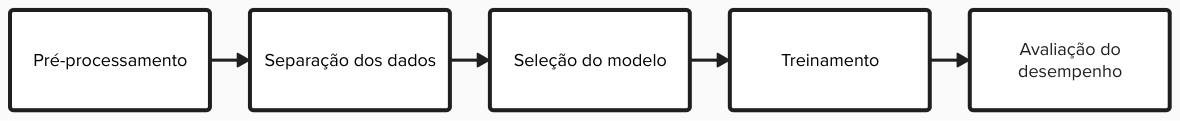
\includegraphics[width=\textwidth]{./02-desenvolvimento/01-machine-learning/imagens/processo.png}
    \caption{Estágios para a construção de um modelo de aprendizagem de máquina.}
    \label{fig:processo}
\end{figure}

\paragraph{Pré-processamento}

O desempenho de um modelo de aprendizagem de máquina depende, em grande medida, da forma como os dados de treinamento são apresentados. Assim é fundamental
uma etapa de processamento inicial para garantir que os padrões mínimos de qualidade dos dados são atendidos. Tarefas de pré-processemento comuns são imputação
de dados faltantes, balanceamento de classes através de \textit{up-sampling} ou \textit{down-sampling}, recodificação de variáveis categóricas e padronização
de variáveis quantitativas \cite{Delgadillo2020}.

\paragraph{Separação dos dados}

A.

\paragraph{Seleção do modelo}

A.

\paragraph{Treinamento}

A.

\paragraph{Avaliação do desempenho}

A.